% Copyright 2004 by Till Tantau <tantau@users.sourceforge.net>.
%
% In principle, this file can be redistributed and/or modified under
% the terms of the GNU Public License, version 2.
%
% However, this file is supposed to be a template to be modified
% for your own needs. For this reason, if you use this file as a
% template and not specifically distribute it as part of a another
% package/program, I grant the extra permission to freely copy and
% modify this file as you see fit and even to delete this copyright
% notice.

\documentclass[11pt]{beamer}
\usepackage{subcaption}
\usepackage[english]{babel}
\usepackage{arydshln}
\usepackage{amsthm}
\usepackage{booktabs}
\usepackage{xcolor}
\usepackage{multirow}
\usepackage{caption}
\usepackage{kotex}
\usepackage{physics}
\usepackage{bibentry}
%\usepackage{mathtools}
\usepackage{natbib}
\bibliographystyle{unsrtnat}
\usepackage{amsmath}
\usepackage{amsfonts}
\usepackage{amssymb}
\usepackage{hyperref}
\hypersetup{
    colorlinks=true,
    linkcolor=black,
    filecolor=magenta,      
    urlcolor=blue,
    pdfpagemode=FullScreen,
    }

 % Top and bottom rules for table


% There are many different themes available for Beamer. A comprehensive
% list with examples is given here:
% http://deic.uab.es/~iblanes/beamer_gallery/index_by_theme.html
% You can uncomment the themes below if you would like to use a different
% one:
%\usetheme{AnnArbor}
%\usetheme{Antibes}
%\usetheme{Bergen}
%\usetheme{Berkeley}
%\usetheme{Berlin}
%\usetheme{Boadilla}
%\usetheme{boxes}
%\usetheme{CambridgeUS}
%\usetheme{Copenhagen}
%\usetheme{Darmstadt}
%\usetheme{default}
%\usetheme{Frankfurt}
%\usetheme{Goettingen}
%\usetheme{Hannover}
%\usetheme{Ilmenau}
%\usetheme{JuanLesPins}
%\usetheme{Luebeck}
\usetheme{Madrid}
%\usetheme{Malmoe}
%\usetheme{Marburg}
%\usetheme{Montpellier}
%\usetheme{PaloAlto}
%\usetheme{Pittsburgh}
%\usetheme{Rochester}
%\usetheme{Singapore}
%\usetheme{Szeged}
%\usetheme{Warsaw}
\usecolortheme{rose}
%%%%%%%%%%%%%%%%%%%%%%%%%%%%%%%%%%%%%%%%%%%%%%%%%%%%
%%         문자에 액센트
%%%%%%%%%%%%%%%%%%%%%%%%%%%%%%%%%%%%%%%%%%%%%%%%%%%%

% % true
% \newcommand{\thetat}{{\theta^t}}
% \newcommand{\pt}{{p^t}}
% \newcommand{\Et}{{\mathbb{E}^t}}
% \newcommand{\Vt}{{\mathbb{V}ar^t}}


% % hat
% \newcommand{\dhat}{\hat{d}}
% \newcommand{\fhat}{\hat{f}}
% \newcommand{\ghat}{\hat{g}}
% \newcommand{\hhat}{\hat{h}}
% \newcommand{\mhat}{\hat{m}}
% \newcommand{\phat}{\hat{p}}
% \newcommand{\uhat}{\hat{u}}
% \newcommand{\vhat}{\hat{v}}
% \newcommand{\xhat}{\hat{x}}
% \newcommand{\yhat}{\hat{y}}
% \newcommand{\Fhat}{\hat{F}}
% \newcommand{\Ghat}{\hat{G}}
% \newcommand{\Hhat}{\hat{H}}
% \newcommand{\Ihat}{\hat{I}}
% \newcommand{\Vhat}{\hat{V}}
% \newcommand{\Xhat}{\hat{X}}
% \newcommand{\Yhat}{\hat{Y}}
% \newcommand{\alphahat}{{\hat{\alpha}}}
% \newcommand{\betahat}{{\hat{\beta}}}
% \newcommand{\gammahat}{{\hat{\gamma}}}
% \newcommand{\etahat}{{\hat{\eta}}}
% \newcommand{\muhat}{{\hat{\mu}}}
% \newcommand{\pihat}{{\hat{\pi}}}
% \newcommand{\phihat}{{\hat{\phi}}}
% \newcommand{\psihat}{{\hat{\psi}}}
% \newcommand{\sigmahat}{{\hat{\sigma}}}
% \newcommand{\thetahat}{{\hat{\theta}}}
% \newcommand{\Sigmahat}{{\hat{\Sigma}}}

% % bar
% \newcommand{\pbar}{\bar{p}}
% \newcommand{\xbar}{\bar{x}}
% \newcommand{\ybar}{\bar{y}}
% \newcommand{\zbar}{\bar{z}}
% \newcommand{\Dbar}{\bar{D}}
% \newcommand{\Tbar}{\bar{X}}
% \newcommand{\Xbar}{\bar{X}}
% \newcommand{\Ybar}{\bar{Y}}
% \newcommand{\Zbar}{\bar{Z}}
% \newcommand{\thetabar}{\bar{\theta}}
% \newcommand{\etabar}{\bar{\eta}}

% % tilde
% \newcommand{\ptilde}{ \tilde{p}}
% \newcommand{\Rtilde}{ \tilde{R}}
% \newcommand{\Vtilde}{ \tilde{V}}
% \newcommand{\Xtilde}{ \tilde{X}}
% \newcommand{\Ytilde}{ \tilde{Y}}
% \newcommand{\betatilde}{ \tilde{\beta}}
% \newcommand{\mutilde}{ \tilde{\mu}}
% \newcommand{\xitilde}{ \tilde{\xi}}
% \newcommand{\thetatilde}{ \tilde{\theta}}
% \newcommand{\sigmatilde}{ \tilde{\sigma}}
% \newcommand{\Sigmatilde}{ \tilde{\Sigma}}
% \newcommand{\Vartilde}{ \tilde{Var}}


% % dot
% \newcommand{\Edot}{ \dot{E}}
% \newcommand{\Idot}{ \dot{I}}
% \newcommand{\Rdot}{ \dot{R}}
% \newcommand{\Sdot}{ \dot{S}}
% \newcommand{\fdot}{ \dot{f}}
% \newcommand{\xdot}{ \dot{x}}


% % bold
% \newcommand{\bfc}{\mathbf{c}}
% \newcommand{\bff}{ \mathbf{f}}
% \newcommand{\bfm}{ \mathbf{m}}
% \newcommand{\bfn}{ \mathbf{n}}
% \newcommand{\bfr}{ \mathbf{r}}
% \newcommand{\bfs}{ \mathbf{s}}
% \newcommand{\bft}{ \mathbf{t}}
% \newcommand{\bfu}{ \mathbf{u}}
% \newcommand{\bfw}{ \mathbf{w}}
% \newcommand{\bfx}{ \mathbf{x}}
% \newcommand{\bfy}{ \mathbf{y}}
% \newcommand{\bfz}{ \mathbf{z}}
% \newcommand{\bfE}{ \mathbf{E}}
% \newcommand{\bfF}{ \mathbf{F}}
% \newcommand{\bfO}{ \mathbf{O}}
% \newcommand{\bfX}{ \mathbf{X}}
% \newcommand{\bfY}{ \mathbf{Y}}
% \newcommand{\bfZ}{\mathbf{Z}}
% \newcommand{\bfzero}{{\bf 0}}
% \newcommand{\bfone}{{\bf 1}}


% % blackboard bold
% \newcommand{\bbC}{{ \mathbb{C}}}
% \newcommand{\bbE}{{ \mathbb{E}}}
% \newcommand{\bbN}{ \mathbb{N}}
% \newcommand{\bbP}{ \mathbb{P}}
% \newcommand{\bbR}{ \mathbb{R}}
% \newcommand{\bbX}{ \mathbb{X}}
% \newcommand{\bbY}{ \mathbb{Y}}
% \newcommand{\bbZ}{ \mathbb{Z}}

% % caligraph
% \newcommand{\calA}{\mathcal{A}}
% \newcommand{\calB}{\mathcal{B}}
% \newcommand{\calC}{\mathcal{C}}
% \newcommand{\calD}{\mathcal{D}}
% \newcommand{\calE}{\mathcal{E}}
% \newcommand{\calF}{\mathcal{F}}
% \newcommand{\calG}{\mathcal{G}}
% \newcommand{\calH}{\mathcal{H}}
% \newcommand{\calL}{\mathcal{L}}
% \newcommand{\calM}{\mathcal{M}}
% \newcommand{\calP}{\mathcal{P}}
% \newcommand{\calQ}{\mathcal{Q}}
% \newcommand{\calS}{\mathcal{S}}
% \newcommand{\calT}{\mathcal{T}}
% \newcommand{\calX}{ \mathcal{X}}
% \newcommand{\calY}{\mathcal{Y}}
% \newcommand{\calZ}{\mathcal{Z}}


% % boldsymbol
% \newcommand{\balpha}{ \boldsymbol{\alpha}}
% \newcommand{\bbeta}{ \boldsymbol{\beta}}
% \newcommand{\bepsilon}{ \boldsymbol{\epsilon}}
% \newcommand{\blambda}{ \boldsymbol{\lambda}}
% \newcommand{\bmu}{ \boldsymbol{\mu}}
% \newcommand{\bnu}{ \boldsymbol{\nu}}
% \newcommand{\bpi}{ \boldsymbol{\pi}}
% \newcommand{\bphi}{ \boldsymbol{\phi}}
% \newcommand{\bpsi}{ \boldsymbol{\psi}}
% \newcommand{\btheta}{ \boldsymbol{\theta}}
% \newcommand{\bomega}{ \boldsymbol{\omega}}
% \newcommand{\bxi}{ \boldsymbol{\xi}}

% \newcommand{\bed}{\begin{itemize}}
% 	\newcommand{\eed}{\end{itemize}}
% \newcommand{\vs}{\vspace}


% \newcommand{\jsum}{\sum_{j=1}^{p}}


% %\newcommand{\bfc}{\mathbf{c}}
% %\newcommand{\bff}{ \mathbf{f}}
% \newcommand{\bfg}{ \mathbf{g}}
% %\newcommand{\bfm}{ \mathbf{m}}
% %\newcommand{\bfn}{ \mathbf{n}}
% \newcommand{\bfp}{ \mathbf{p}}
% %\newcommand{\bfr}{ \mathbf{r}}
% %\newcommand{\bfs}{ \mathbf{s}}
% %\newcommand{\bft}{ \mathbf{t}}
% %\newcommand{\bfu}{ \mathbf{u}}
% \newcommand{\bfv}{ \mathbf{v}}
% %\newcommand{\bfw}{ \mathbf{w}}
% %\newcommand{\bfx}{ \mathbf{x}}
% %\newcommand{\bfy}{ \mathbf{y}}
% %\newcommand{\bfz}{ \mathbf{z}}
% %\newcommand{\bfN}{ \mathbf{N}}
% \newcommand{\bfI}{ \mathbf{I}}
% \newcommand{\bfJ}{ \mathbf{J}}
% %\newcommand{\bfE}{ \mathbf{E}}
% %\newcommand{\bfF}{ \mathbf{F}}
% %\newcommand{\bfO}{ \mathbf{O}}
% %\newcommand{\bfS}{ \mathbf{S}}
% \newcommand{\bfV}{ \mathbf{V}}
% %\newcommand{\bfX}{ \mathbf{X}}
% %\newcommand{\bfY}{ \mathbf{Y}}
% %\newcommand{\bfZ}{\mathbf{Z}}
% %\newcommand{\bfzero}{{\bf 0}}
% %\newcommand{\bfone}{{\bf 1}}
% %\newcommand{\balpha}{ \boldsymbol{\alpha}}
% %\newcommand{\bbeta}{ \boldsymbol{\beta}}
% %\newcommand{\bepsilon}{ \boldsymbol{\epsilon}}
% \newcommand{\bvarepsilon}{ \boldsymbol{\varepsilon}}
% %\newcommand{\blambda}{ \boldsymbol{\lambda}}
% %\newcommand{\bmu}{ \boldsymbol{\mu}}
% %\newcommand{\bnu}{ \boldsymbol{\nu}}
% %\newcommand{\bpi}{ \boldsymbol{\pi}}
% %\newcommand{\bphi}{ \boldsymbol{\phi}}
% %\newcommand{\bpsi}{ \boldsymbol{\psi}}
% %\newcommand{\btheta}{ \boldsymbol{\theta}}
% %\newcommand{\bomega}{ \boldsymbol{\omega}}
% %\newcommand{\bxi}{ \boldsymbol{\xi}}
% \newcommand{\bfeta}{ \boldsymbol{\eta}}
% \newcommand{\bsigma}{ \boldsymbol{\sigma}}
% \newcommand{\bzero}{\boldsymbol{0}}
% \newcommand{\bone}{\boldsymbol{1}}

\newcommand{\rmk}{$\surd$}
\newcommand{\sq}{$\square$}
\newcommand{\N}{\mathbb{N}}
\newcommand{\R}{\mathbb{R}}
\newcommand{\U}{\mathcal{U}}
\newcommand{\V}{\mathcal{V}}
\newcommand{\A}{\mathcal{A}}
\newcommand{\B}{\mathcal{B}}
\newcommand{\C}{\mathcal{C}}
\newcommand{\open}{\underset{open}{\subset}}
\newcommand{\closed}{\underset{closed}{\subset}}
\newcommand{\subsp}{\underset{subsp}{\subset}}
\newcommand{\seq}{\underset{seq}{\subset}}
\newcommand{\cl}{\overline}
\newcommand{\diff}{\,\backslash\,}
\newcommand{\exist}{\exists\,}
\newcommand{\homeo}{\underset{Homeo}{\simeq}}
\newcommand{\floor}[1]{\left\lfloor #1 \right\rfloor}


\title[Mallows Rank Model]{
Bayesian Mallows Model for Rank Data}

% A subtitle is optional and this may be deleted
%\subtitle{Optional Subtitle}

\author{
장태영
}
% - Give the names in the same order as the appear in the paper.
% - Use the \inst{?} command only if the authors have different
%   affiliation.

\institute[서울대학교] % (optional, but mostly needed)
{
  서울대학교\\
  통계학과, 베이즈통계 연구실
}
% - Use the \inst command only if there are several affiliations.
% - Keep it simple, no one is interested in your street address.

\date{2021. 11. 12}
% - Either use conference name or its abbreviation.
% - Not really informative to the audience, more for people (including
%   yourself) who are reading the slides online

% \subject{Bayesian Nonparametric Function Estimation}
% This is only inserted into the PDF information catalog. Can be left
% out.

% If you have a file called "university-logo-filename.xxx", where xxx
% is a graphic format that can be processed by latex or pdflatex,
% resp., then you can add a logo as follows:

% \pgfdeclareimage[height=0.5cm]{university-logo}{university-logo-filename}
% \logo{\pgfuseimage{university-logo}}

\usepackage{graphicx}
\graphicspath{ {./images/} } % 그림이 들어있는 디렉토리 지정.

% Delete this, if you do not want the table of contents to pop up at
% the beginning of each subsection:
\AtBeginSection[]
{
  \begin{frame}<beamer>{CONTENTS}
    \tableofcontents[currentsection]
  \end{frame}
}

% Let's get started
\begin{document}

\begin{frame}
  \titlepage
\end{frame}

\begin{frame}{CONTENTS}
  \tableofcontents
  % You might wish to add the option [pausesections]
\end{frame}

\section{Motivation}
\begin{frame}{Motivation}
\begin{itemize}
    \item Ranking and comparing items
    \begin{itemize}
        \item Crucial for collecting information about preferences in many areas from marketing to politics
        \item Netflix, Spotify, 배달의 민족, ...  
    \end{itemize}
\end{itemize}
\end{frame}

\begin{frame}{Example data}
    \begin{figure}[h]
        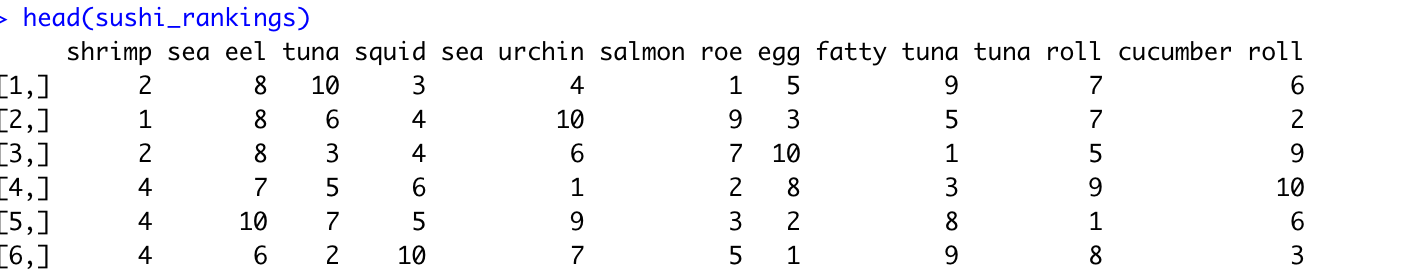
\includegraphics[width=10cm]{sushidata.png}
        \centering
    \end{figure}
\end{frame}

\begin{frame}{What we want to do?}
    \begin{itemize}
        \item Find consensus ranking of the items
        \item Extensions of model for pairwise comparisons, preference prediction and clustering.
    \end{itemize}
\end{frame}

\section{A Bayesian Mallows model for complete rankings}
\begin{frame}{Elementary settings}
\begin{itemize}
    \item Setting : $n$ items and $N$ assessors. $\mathbf{R}_j\in \mathcal{P}_n$ denotes the ranking(the full set of ranks given to the $n$ items) of assessor $j$ for each $j=1,\cdots, N$. ($\mathcal{P}_n$ is a permutation set)
    \item $d(\cdot\;,\; \cdot): \mathcal{P}_n\times \mathcal{P}_n\rightarrow [0,\infty)$ is a distance function between two rankings.
    \begin{itemize}
        \item Kendall distance : number of pairs of distinct elements whose order in the two rankings are the opposite.
        \item Footrule distance : $\ell_1$ distance
        \item Spearman's distance : $\ell_2$ distance 
    \end{itemize}
\end{itemize} 
\end{frame}

\begin{frame}{Mallows model}
\begin{itemize}
    \item Mallows model is a class of non-uniform joint distributions for a ranking $\mathbf{r}$ on $\mathcal{P}_n$. $$P(\mathbf{r}|\alpha, \boldsymbol{\rho})=Z_n(\alpha, \boldsymbol{\rho})^{-1}\exp\{-\frac{\alpha}{n}d(\mathbf{r}, \boldsymbol{\rho})\}I(\mathbf{r}\in \mathcal{P}_n) $$
    \item $\boldsymbol{\rho}\in \mathcal{P}_n$ is the latent consensus ranking. 
    \item $\alpha>0$ is a scale (or precision) parameter. \\i.e. $\alpha$ represents the level of agreement between assesssors, so that as $\alpha$ gets larger, ranking $\mathbf{r}$ aggregates more to $\boldsymbol{\rho}$ 
    \item $Z_n(\alpha, \boldsymbol{\rho})=\sum_{\mathbf{r}\in \mathcal{P}_n}e^{-\frac{\alpha}{n}d(\mathbf{r},\boldsymbol{\rho})}$ is the partition function.
    \begin{itemize}
        \item In physics, a `partition function' describes the statistical properties of a system in thermodynamic equilibrium. (Source : Wikipedia)
        \item Here, just consider this as a normalizing factor.
    \end{itemize}
\end{itemize} 
\end{frame}


\begin{frame}{Likelihood function}
\begin{itemize}
    \item Assume that observed rankings $\mathbf{R}_1, \cdots, \mathbf{R}_N$ are conditionally independent given $\alpha$ and $\boldsymbol{\rho}$ and each of them is distributed according to the Mallows model with these parameters.
    \item Likelihood takes the form as \begin{equation*}P(\mathbf{R}_1, \cdots, \mathbf{R}_N|\alpha, \boldsymbol{\rho})= Z_n(\alpha, \boldsymbol{\rho})^{-N}\exp\{-\frac{\alpha}{n}\sum_{j=1}^N d(\mathbf{R}_j, \boldsymbol{\rho})\}\prod_{j=1}^N I(\mathbf{R}_j\in \mathcal{P}_n) \end{equation*}
    \item For large $n$, finding the MLE of $\boldsymbol{\rho}$ given fixed $\alpha$ is not feasible because the space of permutations $\mathcal{P}_n$ has $n!$ elements. 
\end{itemize} 
\end{frame}

\begin{frame}{Right-invariant distance and partition function}
\begin{itemize}
    \item For any right-invariant distance, it holds $d(\mathbf{r}_1, \mathbf{r}_2)=d(\mathbf{r}_1 \mathbf{r}_2^{-1}, \mathbf{1}_n)$ where $\mathbf{1}_n=\{1,2,\cdots,n\}$ and $\mathbf{r}_1 \mapsto \mathbf{r}_1 \mathbf{r}_2^{-1}$ is relabelling map. Note that a right-invariant distance is unaffected by a relabelling of the items.
    \item Partition function $Z_n(\alpha, \boldsymbol{\rho})$ does not depend on $\boldsymbol{{\rho}}$. 
    \begin{align*}
    \because Z_n(\alpha, \boldsymbol{\rho}) &= \sum_{\mathbf{r}\in \mathcal{P}_n}\exp\{-\frac{\alpha}{n}d(\mathbf{r},\boldsymbol{\rho})\} = \sum_{\mathbf{r}\in \mathcal{P}_n}\exp\{-\frac{\alpha}{n}d(\mathbf{r} \boldsymbol{\rho}^{-1}, \mathbf{1}_n)\} \\ &=\sum_{\mathbf{r'}\in \mathcal{P}_n}\exp\{-\frac{\alpha}{n}d(\mathbf{r'},\mathbf{1}_n)\} \\ Z_n(\alpha, \boldsymbol{\rho}) &= Z_n(\alpha)=\sum_{\mathbf{r}\in \mathcal{P}_n}\exp\{-\frac{\alpha}{n}d(\mathbf{r},\mathbf{1}_n)\}
    \end{align*}
\end{itemize}
\end{frame}

\begin{frame}{Right-invariant distance and partition function}
\begin{itemize}
    \item For some choice of right-invariant distance like Kendall distance, the partition function can be analytically computed. 
    \item But there are important and natural right-invariant distances for which the computation of the partition function is not feasible, such as the footrule distance and the Spearman's distance.
\end{itemize}
\end{frame}

\begin{frame}{Prior distributions}
    \begin{itemize}
        \item Assume a priori that $\alpha$ and $\boldsymbol{\rho}$ are independent
        \item In this paper, the uniform prior $\pi(\boldsymbol{\rho})=\frac{1}{n!}I(\boldsymbol{\rho}\in \mathcal{P}_n)$ is employed.
        \item Also, for the scale parameter, this paper used a truncated exponential prior with density $\pi(\alpha | \lambda)=\lambda e^{-\lambda \alpha}I(\alpha\in [0, \alpha_{max}])/(1-e^{-\lambda \alpha_{max}})$ where the cut-off point $\alpha_{max}<\infty$ is large compared to the values supported by the data. In practice, in the computations involving the sampling of values for $\alpha$, truncation was never applied. We assign $\lambda$ a fixed value close to zero, implying a prior density for $\alpha$ which is quite flat.
        \begin{itemize}
            \item In short, prior $\alpha \sim Exp(\frac{1}{\lambda})$ with small $\lambda$ is used practically for $\alpha$. 
        \end{itemize}
    \end{itemize}
\end{frame}

\begin{frame}{Posterior distributions}
\begin{itemize}
    \item The posterior distribution for $\boldsymbol{\rho}$ and $\alpha$ is given by
    \begin{equation} \label{posterior}
        P(\boldsymbol{\rho}, \alpha| \mathbf{R}_1, \cdots, \mathbf{R}_N)\propto \frac{\pi(\boldsymbol{\rho})\pi(\alpha)}{Z_n(\alpha)^N} \exp \big\{-\frac{\alpha}{n}\sum_{j=1}^N d(\mathbf{R}_j, \boldsymbol{\rho})\big\}
    \end{equation}
    \item The purpose of MCMC algorithm following is to obtain samples from this posterior.
\end{itemize}
\end{frame}

\begin{frame}{Metropolis-Hastings algorithm}
\begin{itemize}
    \item A general form of the Metropolis Hastings algorithm is as follows : \\ Target probability distribution is $p_0(x)$ for r.v. $X$. Given a current value $x^{(s)}$ of $X$, 
        \begin{enumerate}
            \item Generate $x^{*}$ from a proposal distribution $J_s(x^{*}|x^{(s)})$
            \item Compute the acceptance ratio $$ r=\frac{p_0(x^*)}{p_0(x^{(s)})}\, /\, \frac{J_s(x^*|x^{(s)})}{J_s(x^{(s)}|x^*)} = \frac{p_0(x^*)}{p_0(x^{(s)})}\frac{J_s(x^{(s)}|x^*)}{J_s(x^*|x^{(s)})} $$
            \item set $x^{(s+1)}$ to $x^*$ with probability $\min (1, r)$ \\ i.e. Sample $u\sim unif(0,1)$ and then if $u<r$ set $x^{(s+1)}=x^*$, else set $x^{(s+1)}=x^{(s)}$
        \end{enumerate}
\end{itemize}
\end{frame}

\begin{frame}{Metropolis-Hastings algorithm}
\begin{itemize}
    \item The primary restriction placed on $J_s(x^*|x^{(s)})$ is that it does not depend on values in the sequence previous to $x^{(s)}$ so that the algorithm generates a Markov chain.
    \item By Ergodic Thm, the empirical distribution of samples generated from such a Markov chain will converge to the stationary distribution (of the Markov chain), which agrees with the target distribution.
    \item Source : Hoff 2009. (textbook)
\end{itemize}
\end{frame}

\begin{frame}{Metropolis-Hastings Algorithm for Complete Rankings}
\begin{itemize}
    \item To obtain samples from the posterior distribution \eqref{posterior}, we alternate between two steps.
    \begin{enumerate}
        \item Given $\alpha$ and $\boldsymbol{\rho}$, update $\boldsymbol{\rho}$ by proposing $\boldsymbol{\rho}'$
        \item Then, given $\alpha$ and $\boldsymbol{\rho}'$, update $\alpha$ by proposing $\alpha'$
    \end{enumerate}
\end{itemize}
\end{frame}

\begin{frame}{Updating $\boldsymbol{\rho}$}
\begin{itemize}
    \item Leap-and-Shift Proposal(L\&S)
    \item Leap step
        \begin{enumerate}
            \item Fix an integer $L\in \{1,2,\cdots, \floor{\frac{n-1}{2}}\}$ \\
            (which is a tuning parameter for MCMC algorithm)
            \item Draw a random number $u\sim Unif\{1,2,\cdots, n\}$
            \item Define $\mathcal{S}\subset \{1,2,\cdots, n\}$ by $\mathcal{S}=\big[\max (1, \rho_u-L), \min (n, \rho_u+L)\big]\diff\{\rho_u\}$
            \item Draw a random number $r\sim Unif(\mathcal{S})$
            \item Let $\boldsymbol{\rho}^*\in \{1,2,\cdots, n\}^n$ have elements $\begin{cases}
            \rho_i^*=\rho_i & i\in \{1,2,\cdots,n\}\diff \{u\} \\\rho_u^*=r \end{cases}$
        \end{enumerate}
\end{itemize}
\end{frame}

\begin{frame}{Updating $\boldsymbol{\rho}$}
\begin{itemize}
    \item Shift step
    \begin{enumerate}
        \item Let $\Delta=\rho_u^*-\rho_u$. Note that $\Delta\neq 0$ 
        \item Define the proposed $\boldsymbol{\rho}'\in \mathcal{P}_n$ by below :
        \begin{enumerate}
            \item If $\Delta>0$ then 
            $$\begin{cases}
                \rho_u'=\rho_u^* \\ \rho_i'=\rho_i-1 & if \; \rho_u<\rho_i\leq \rho_u^* \\ \rho_i'=\rho_i & otherwise
            \end{cases} $$
            \item If $\Delta<0$ then 
            $$\begin{cases}
                \rho_u'=\rho_u^* \\ \rho_i'=\rho_i+1 & if \; \rho_u>\rho_i\geq \rho_u^* \\ \rho_i'=\rho_i & otherwise
            \end{cases} $$
        \end{enumerate} 
    \end{enumerate}
\end{itemize}
\end{frame}

\begin{frame}{Updating $\boldsymbol{\rho}$}
\begin{itemize}
    \item Example of Leap and Shift proposal
    \begin{figure}
        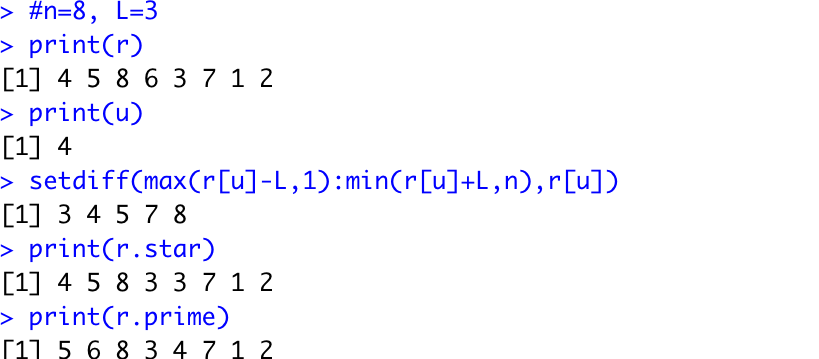
\includegraphics{LeapAndShift.png}
    \end{figure}
\end{itemize}
\end{frame}

\begin{frame}{Updating $\boldsymbol{\rho}$}
\begin{itemize}
    \item The probability mass function associated to the transition
    \begin{figure}
        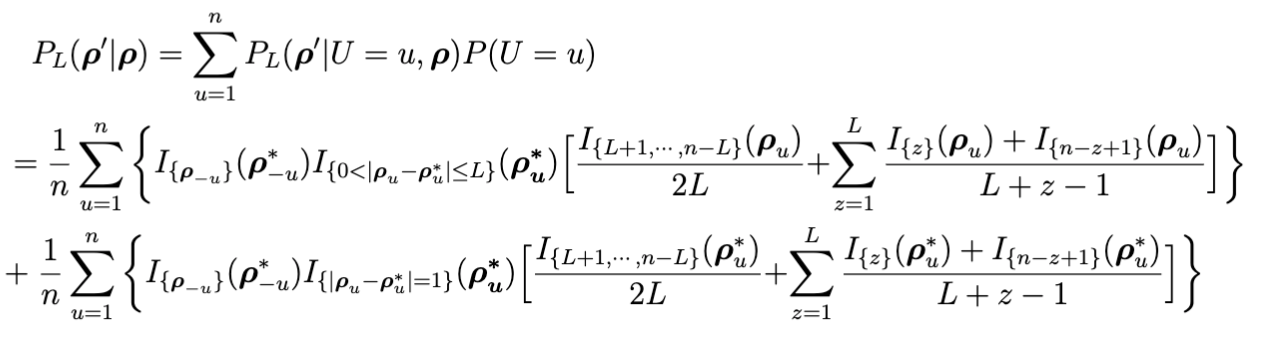
\includegraphics[width=11cm]{transitionProb.png}
    \end{figure}
\end{itemize}
\end{frame}

\begin{frame}{Updating $\boldsymbol{\rho}$}
\begin{itemize}
    \item Simple representation for the transition probability
        \begin{itemize}
            \item As we calculate $P(\boldsymbol{\rho}'|\boldsymbol{\rho})$, we should consider two random draws
            \begin{itemize}
                \item Draw $u\sim Unif\{1,2,\cdots, n\}$
                \item For $S$ dependent on $\boldsymbol{\rho}_u$, draw $r\sim Unif(S)$
                \item The other works including shift step involve no randomness.
            \end{itemize}
            \item Simply put, $P(\boldsymbol{\rho}'|\boldsymbol{\rho})=\frac{1}{n}\cdot\frac{1}{|S|}$ for many cases.
            \item However, if $|\boldsymbol{\rho}_u'-\boldsymbol{\rho}_u|=1$ then we should consider something more. 
            \item When $|\boldsymbol{\rho}_u'-\boldsymbol{\rho}_u|>1$ then $u$ is the only possible index that proposes $\boldsymbol{\rho}'$ from $\boldsymbol{\rho}$. On the other hand, when $|\boldsymbol{\rho}_u'-\boldsymbol{\rho}_u|=1$, there must be only one index $u'$ other than $u$ s.t. $|\boldsymbol{\rho}_{u'}'-\boldsymbol{\rho}_{u'}|=1$ so that $u'$ can also proposes $\boldsymbol{\rho}'$ from $\boldsymbol{\rho}$.
            \item In this special case, $P(\boldsymbol{\rho}'|\boldsymbol{\rho})=\frac{1}{n}\cdot\frac{1}{|S|}+\frac{1}{n}\cdot\frac{1}{|S'|}$ where $S$ is produced from drawing $u$ and $S'$ is produced from drawing $u'$
        \end{itemize}
\end{itemize}
\end{frame}

\begin{frame}{Updating $\boldsymbol{\rho}$}
\begin{itemize}
    \item example of leap and shift proposal  when $|\boldsymbol{\rho}_u'-\boldsymbol{\rho}_u|=1$
    \begin{figure}
        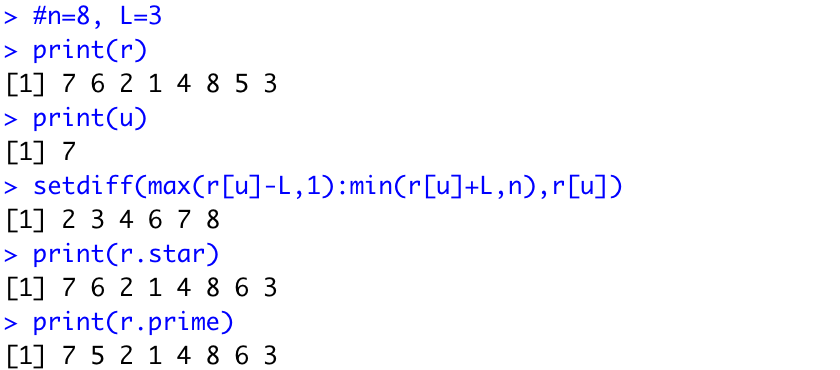
\includegraphics{LSproposal1.png}
    \end{figure}
\end{itemize}
\end{frame}

\begin{frame}{Updating $\boldsymbol{\rho}$}
\begin{itemize}
    \item Using this logic, we can rewrite the equality about $P_L(\boldsymbol{\rho}'|\boldsymbol{\rho})$ as the following 
    \begin{align*}
        P_L(\boldsymbol{\rho}'|\boldsymbol{\rho}) &= \sum_{u=1}^n P_L(\boldsymbol{\rho}'|U=u, \boldsymbol{\rho})P(U=u) \\ &= \frac{1}{n}\sum_{u=1}^n I(\boldsymbol{\rho}', \boldsymbol{\rho}, u) \frac{1}{|S^{(u)}|}
    \end{align*}
    where $I(\boldsymbol{\rho}', \boldsymbol{\rho}, u)$ is an indicator for possibility of proposal from $\boldsymbol{\rho}$ to $\boldsymbol{\rho}'$ given $u$ is drawed and $S^{(u)}$ is the set $S$ given $u$ is drawed \\ If $\boldsymbol{\rho}'$ is proposed from $\boldsymbol{\rho}$ then typically $I(\boldsymbol{\rho}', \boldsymbol{\rho}, u)=1$ for only one $u$ but if $|\boldsymbol{\rho}_u'-\boldsymbol{\rho}_u|=1$ then $I(\boldsymbol{\rho}', \boldsymbol{\rho}, u')=1$ also holds for another $u'$ different from $u$
\end{itemize}
\end{frame}

\begin{frame}{Updating $\boldsymbol{\rho}$}
\begin{itemize}
    \item The acceptance probability when updating $\boldsymbol{\rho}$ is 
        $\min\{1, r\}$ where $r$ is given as 
        \begin{align*}
            r &=\frac{P(\boldsymbol{\rho}', \alpha | \mathbf{R})}{P(\boldsymbol{\rho}, \alpha | \mathbf{R})}\cdot \frac{P_L(\boldsymbol{\rho}|\boldsymbol{\rho}')}{P_L(\boldsymbol{\rho}'|\boldsymbol{\rho})} \\ &= \frac{P_L(\boldsymbol{\rho}|\boldsymbol{\rho}')}{P_L(\boldsymbol{\rho}'|\boldsymbol{\rho})} \cdot \frac{\pi(\boldsymbol{\rho}')}{\pi(\boldsymbol{\rho})}\exp\big\{-\frac{\alpha}{n}\sum_{j=1}^N \big[d(\mathbf{R}_j, \boldsymbol{\rho}')-d(\mathbf{R}_j, \boldsymbol{\rho})\big] \big\}
        \end{align*} 
    \item Leap and shift proposal is not a symmetric proposal distribution. 
    \item The term $\sum_{j=1}^N \big[d(\mathbf{R}_j, \boldsymbol{\rho}')-d(\mathbf{R}_j, \boldsymbol{\rho})\big]$ above can be computed efficiently since most elements of $\boldsymbol{\rho}$ and $\boldsymbol{\rho}'$ are equal and we can put aside indices $i$ s.t. $\rho_i=\rho'_i$
\end{itemize}
\end{frame}

\begin{frame}{Updating $\alpha$}
\begin{itemize}
    \item Sample a proposal $\alpha '$ from a lognormal distribution $\log\mathcal{N}(\log(\alpha), \sigma_\alpha^2)$ \\ $\sigma_\alpha^2$ is a tuning parameter for MCMC algorithm.
    \item Note that $X\sim \log\mathcal{N}(\mu, \sigma^2)\Leftrightarrow Y=\log X\sim N(\mu, \sigma^2)$ \\ The pdf of $X\sim \log\mathcal{N}(\log(\mu), \sigma^2)$ is written as $$f(x ; \mu, \sigma)=\frac{1}{\sqrt{2\pi \sigma^2}}\exp\bigl(-\frac{1}{2\sigma^2}(\log x -\log \mu)^2 \bigr)\frac{1}{x}\,I(x>0)$$
    \item The probability density function associated to the transition is $$J(\alpha'|\alpha)=\frac{1}{\sqrt{2\pi \sigma_\alpha^2}}\exp\bigl(-\frac{1}{2\sigma_\alpha^2}(\log \alpha' -\log \alpha)^2 \bigr)\frac{1}{\alpha'}$$
    Accordingly, we have the ratio $\frac{J(\alpha'|\alpha)}{J(\alpha|\alpha')}=\frac{\alpha}{\alpha'}$ 
\end{itemize}
\end{frame}

\begin{frame}{Updating $\alpha$}
\begin{itemize}
    \item Acceptance probability is $\min\{1, r\}$ where $r$  is given as 
    \begin{align*}
        r &= \frac{P(\boldsymbol{\rho}, \alpha' | \mathbf{R})}{P(\boldsymbol{\rho}, \alpha | \mathbf{R})} \,/\, \frac{J(\alpha'|\alpha)}{J(\alpha|\alpha')} \\ &= \frac{\alpha'}{\alpha}\frac{\pi(\alpha')}{\pi(\alpha)}\frac{Z_n(\alpha)^N}{Z_n(\alpha')^N}\exp \big\{-\frac{\alpha'-\alpha}{n}\sum_{j=1}^N d(\mathbf{R}_j, \boldsymbol{\rho})\big\}
    \end{align*}
    \item Additional parameter $\alpha_{jump}$ can be used to update $\alpha$ only every $\alpha_{jump}$ updates of $\boldsymbol{\rho}$
\end{itemize}
\end{frame}

\section{Approximating the Partition Function $Z_n(\alpha)$ via Off-line Importance Sampling}
\begin{frame}{Motivation for approximating $Z_n(\alpha)$}
\begin{itemize}
    \item Notice that MCMC algorithm to obtain samples from the posterior distribution, we need to know the value of $Z_n(\alpha)$ which appears in acceptance probability for updating $\alpha$
    \item The partition function $Z_n(\alpha)$ is available in close form for Kendall's, Hamming, and Cayley distances.
    \item But this is not the case for footrule and Spearman distances.
\end{itemize}
\end{frame}

\begin{frame}{$Z_n(\alpha)$ unavailable for some useful distances}
\begin{itemize}
    \item $Z_n(\alpha)=\sum_{\mathbf{r}\in \mathcal{P}_n}\exp\{-\frac{\alpha}{n}d(\mathbf{r},\mathbf{1}_n)\}$
    \item Note that $d(\mathbf{r}, \mathbf{1}_n)$ takes only the finite number of discrte values $\mathcal{D}=\{d_1, \cdots , d_a\}$ where $a$ depends on $n$ and distance $d(\cdot\,,\,\cdot)$
    \item It can be rewritten as $$Z_n(\alpha)=\sum_{d_i\in \mathcal{D}}|L_i|\exp\{-\frac{\alpha}{n}d_i\} $$ where $L_i=\{\mathbf{r}\in \mathcal{P}_n : d(\mathbf{r}, \mathbf{1}_n)=d_i\}$
    \item To compute $Z_n(\alpha)$ we only need $|L_i|$ for all values $d_i\in \mathcal{D}$
\end{itemize}
\end{frame}

\begin{frame}{$Z_n(\alpha)$ unavailable for some useful distances}
\begin{itemize}
    \item In the case of footrule distance
    \begin{itemize}
        \item $\mathcal{D}$ includes all even numbers from $0$ to $\floor{n^2/2}$
        \item $|L_i|$ corresponds to the sequence A061869 available for $n\leq 50$ on the OEIS(Online Encyclopedia of Integer Sequences)
    \end{itemize}
    \item In the case of Spearman's distance
    \begin{itemize}
        \item $\mathcal{D}$ includes all even numbers from $0$ to $2\binom{n}{3}$
        \item $|L_i|$ corresponds to the sequence A175929 available for $n\leq 14$ on the OEIS
    \end{itemize}
    \item What about the case where $n$ is large?
\end{itemize}
\end{frame}

\begin{frame}{Approximation of $Z_n(\alpha)$}
\begin{itemize}
    \item To handle these cases, we propose an approximation of the partition function $Z_n(\alpha)$ based on importance sampling. 
    \item Recall that given right-invarant distances, the partition function does not depend on $\boldsymbol{\rho}$. 
\end{itemize}
\end{frame}

\begin{frame}{Off-line approximation}
\begin{itemize}
    \item Obtain an off-line approximation of the partition function on a gird of $\alpha$ values. 
    \begin{itemize}
        \item In computer science, an online algorithm is one that can process its input piece-by-piece in a serial fashion, i.e. in the order that the input is fed to the algorithm, without having the entire input available from the start.
        \item In contrast, an offline algorithm is given the whole problem data from the beginning and is required to output an answer which solves the problem at hand. \\ (Source : Wikipedia \href{https://en.wikipedia.org/wiki/Online_algorithm}{Online Algorithm})
    \end{itemize}
    \item Then interpolate it to yield an estimate of $Z_n(\alpha)$ over a continuous range and read off needed values to compute the acceptance probabilities rapidly.
\end{itemize}
\end{frame}

\begin{frame}{Importance sampling}
\begin{itemize}
    \item Suppose our goal is estimate $\mu=E_p[f(X)]$ \\ i.e. the expected value of $f(X)$ under $X\sim p$
    \item For a probability density $q$ other than $p$, we can calculate that 
    \begin{align*} 
        \mu &=E_p[f(X)]=\int f(x)p(x)\, dx \\ &=\int \frac{f(x)p(x)}{q(x)}q(x)\,dx=E_q\Big[\frac{f(X)p(X)}{q(X)}\Big] 
    \end{align*} 
    i.e. $\mu$ equals the expected value of $\frac{f(X)p(X)}{q(X)}$ under $X\sim q$
    \item The importance sampling estimate of $\mu$ is $$\hat \mu_q =\frac{1}{K}\sum_{k=1}^K \frac{f(X_i)p(X_i)}{q(X_i)} \quad \; where \; X_i\sim q$$
\end{itemize}
\end{frame}

\begin{frame}{Importance sampling}
\begin{itemize}
    \item The basic idea of importance sampling is to sample the states from a different distribution to lower the variance of estimation of $\mu$ or when sampling from original density $p$ is difficult.
    \item Reference : Wikipedia and \href{https://statweb.stanford.edu/~owen/mc/Ch-var-is.pdf}{Lecture note from standford.edu}
\end{itemize}
\end{frame}

\begin{frame}{Approximate $Z_n(\alpha)$ using IS approach}
\begin{itemize}
    \item For $K$ rank vectors $\mathbf{R}^1,\cdots, \mathbf{R}^K$ sampled from an IS auxiliary distributution $q(\mathbf{R})$, the unbiased IS estimate of $Z_n(\alpha)$ is given by 
    \begin{equation} \label{ISapproximate}
        \hat{Z}_n(\alpha)=\frac{1}{K}\sum_{k=1}^K \exp\big\{-\frac{\alpha}{n}d(\mathbf{R}^k, \mathbf{1}_n) \big\}\frac{1}{q(\mathbf{R}^k)}
    \end{equation} 
\end{itemize}
\end{frame}

\begin{frame}{Approximate $Z_n(\alpha)$ using IS approach}
\begin{itemize}
    \item IS estimate of $Z_n(\alpha)$ in \eqref{ISapproximate} is derived as the following
    \begin{align*}
        Z_n(\alpha)&=\sum_{\mathbf{R}\in \mathcal{P}_n}\exp\{-\frac{\alpha}{n}d(\mathbf{R},\mathbf{1}_n)\} =\sum_{\mathbf{R}\in \mathcal{P}_n}\frac{1}{P(\mathbf{R})}\exp\{-\frac{\alpha}{n}d(\mathbf{R},\mathbf{1}_n)\}P(\mathbf{R}) \\ &=E_{R\sim P(R)}\Big[ \frac{1}{P(\mathbf{R})}\exp\{-\frac{\alpha}{n}d(\mathbf{R},\mathbf{1}_n)\}\Big] = E_{R\sim P(R)}\big[f(\mathbf{R}) \big]
    \end{align*}
    where $f(\mathbf{R})=\frac{1}{P(\mathbf{R})}\exp\{-\frac{\alpha}{n}d(\mathbf{R},\mathbf{1}_n)\}$ \\and $P(\mathbf{R})$ is abbreviation of $P(\mathbf{R}|\alpha, \mathbf{1}_n)$
    \begin{equation*}
        \hat{Z}_n(\alpha)=\frac{1}{K}\sum_{k=1}^K \frac{f(\mathbf{R}^k)P(\mathbf{R}^k)}{q(\mathbf{R}^k)} =\frac{1}{K}\sum_{k=1}^K \exp\big\{-\frac{\alpha}{n}d(\mathbf{R}^k, \mathbf{1}_n) \big\}\frac{1}{q(\mathbf{R}^k)}
    \end{equation*}
    where $\mathbf{R}^k\sim q(\mathbf{R})$ for each $k=1, \cdots , K$
\end{itemize}
\end{frame}

\begin{frame}{Approximate $Z_n(\alpha)$ using IS approach}
\begin{itemize}
    \item We shall use the following psuedo-likelihood approximation for $q(\mathbf{R})$
    \item While we cannot sample $\mathbf{R}$ from $P(\mathbf{R}|\alpha, \mathbf{1}_n)$ ($\because$ we don't know the value of $Z_n(\alpha)$) it must be computationally feasible to sample $\mathbf{R}$ from $q(\mathbf{R})$.
    \item The more $q(\mathbf{R})$ resembles the Mallows likelihood $P(\mathbf{R}| \alpha, \mathbf{1}_n)$, the smaller is the variance of $\hat{Z}_n(\alpha)$. 
\end{itemize}
\end{frame}

\begin{frame}{Psuedo-likelihood approximation for $q(\mathbf{R})$}
\begin{itemize}
    \item[1] Sample $(i_1, \cdots, i_n)\in \mathcal{P}_n$, which gives the order of the psuedo-lieklihood factorization.
    \item[2] Factorization is given as 
    \begin{multline*}
        P(\mathbf{R}|\mathbf{1}_n)=P(R_{i_n}|\mathbf{1}_n)P(R_{i_{n-1}}|R_{i_n}, \mathbf{1}_n)\cdots P(R_{i_2}|R_{i_3}, \cdots, R_{i_n}, \mathbf{1}_n)\\P(R_{i_1}|R_{i_2}, \cdots, R_{i_n}, \mathbf{1}_n)
    \end{multline*}      
\end{itemize}
\end{frame}

\begin{frame}{Psuedo-likelihood approximation for $q(\mathbf{R})$}
\begin{itemize}
    \item[3] The conditional distributions are given by
    \begin{figure}[h]
        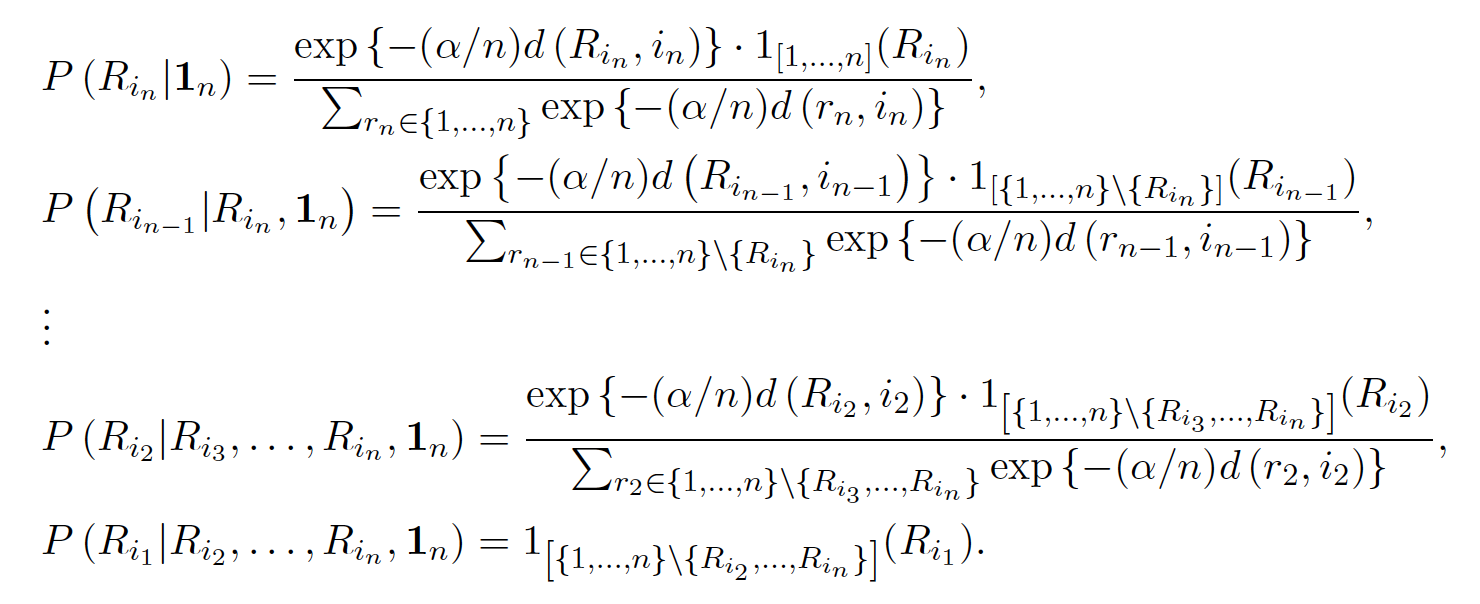
\includegraphics[width=10cm]{ConDist.png}
    \end{figure}
    Each factor is a simple univariate distribution. 
\end{itemize}
\end{frame}

\begin{frame}{Psuedo-likelihood approximation for $q(\mathbf{R})$}
\begin{itemize}
    \item[4] For given value of $\alpha$, sample $R_{i_n}$ first, and then conditionally on that, $R_{i_{n-1}}$ and so on. The $k$-th full sample $\mathbf{R}^k$ has probability 
    \begin{equation*}
        q(\mathbf{R}^k)=P(R_{i_n}^k|\mathbf{1}_n)P(R_{i_{n-1}}^k|R_{i_n}^k, \mathbf{1}_n)\cdots P(R_{i_2}^k|R_{i_3}^k, \cdots, R_{i_n}^k, \mathbf{1}_n)
    \end{equation*} 
    \item[5] Iterate this process $K$ times to calculate $\hat{Z}_n(\alpha)$ as in \eqref{ISapproximate}
    \begin{itemize}
        \item[\rmk] Keeping the psuedo-likelihood with the same distance as the one in the target was most accurate and efficient so we shall use the distance in \eqref{ISapproximate} as same as the distance in \eqref{posterior}. 
    \end{itemize} 
\end{itemize}
\end{frame}

\begin{frame}{Estimate of $Z_n(\alpha)$ over a continuous range}
\begin{itemize}
    \item Over a discrete grid of 100 equally spaced $\alpha$ values between 0.01 and 10 (this is the range of $\alpha$ which turned out to be relevant in all our applications, typically $\alpha<5$), we produce a smooth partition function simply using a polynomial of degree 10.
    \item What we have is 100 data points of $(\alpha^{(i)}, \hat Z_n(\alpha^{(i)}))$'s. A smooth partition function is produced by fitting multiple linear regression for the model $$\log \hat Z_n(\alpha)=\beta_0+\beta_1 \alpha+\beta_2 \alpha^2+\cdots+\beta_{10} \alpha^{10}$$ so that only thing we should store before implementing MCMC for the partition function is those estimated beta parameter values.
\end{itemize}
\end{frame}

\begin{frame}{Effect of approximation on the MCMC}
\begin{itemize}
    \item Theoretical results about the convergence of the MCMC when using the IS approximation of the partition function should be given. 
    \item Algorithm using $\hat{Z}_n$ instead of $Z_n$ converges to the posterior distribution proportional to \begin{equation*} \frac{1}{\hat{C}(\mathbf{R})}\frac{\pi(\boldsymbol{\rho})\pi(\alpha)}{\hat{Z}_n(\alpha)^N} \exp \big\{-\frac{\alpha}{n}\sum_{j=1}^N d(\mathbf{R}_j, \boldsymbol{\rho})\big\} \end{equation*} where the normalizing factor $\hat{C}(\mathbf{R})=\int\sum_{\boldsymbol{\rho}\in \mathcal{P}_n}\frac{\pi(\boldsymbol{\rho})\pi(\alpha)}{\hat{Z}_n(\alpha)^N} \exp \big\{-\frac{\alpha}{n}\sum_{j=1}^N d(\mathbf{R}_j, \boldsymbol{\rho})\big\}\, d\alpha $
\end{itemize}
\end{frame}

\begin{frame}{Studying the effect of approximation by simulations}
    \begin{figure}
        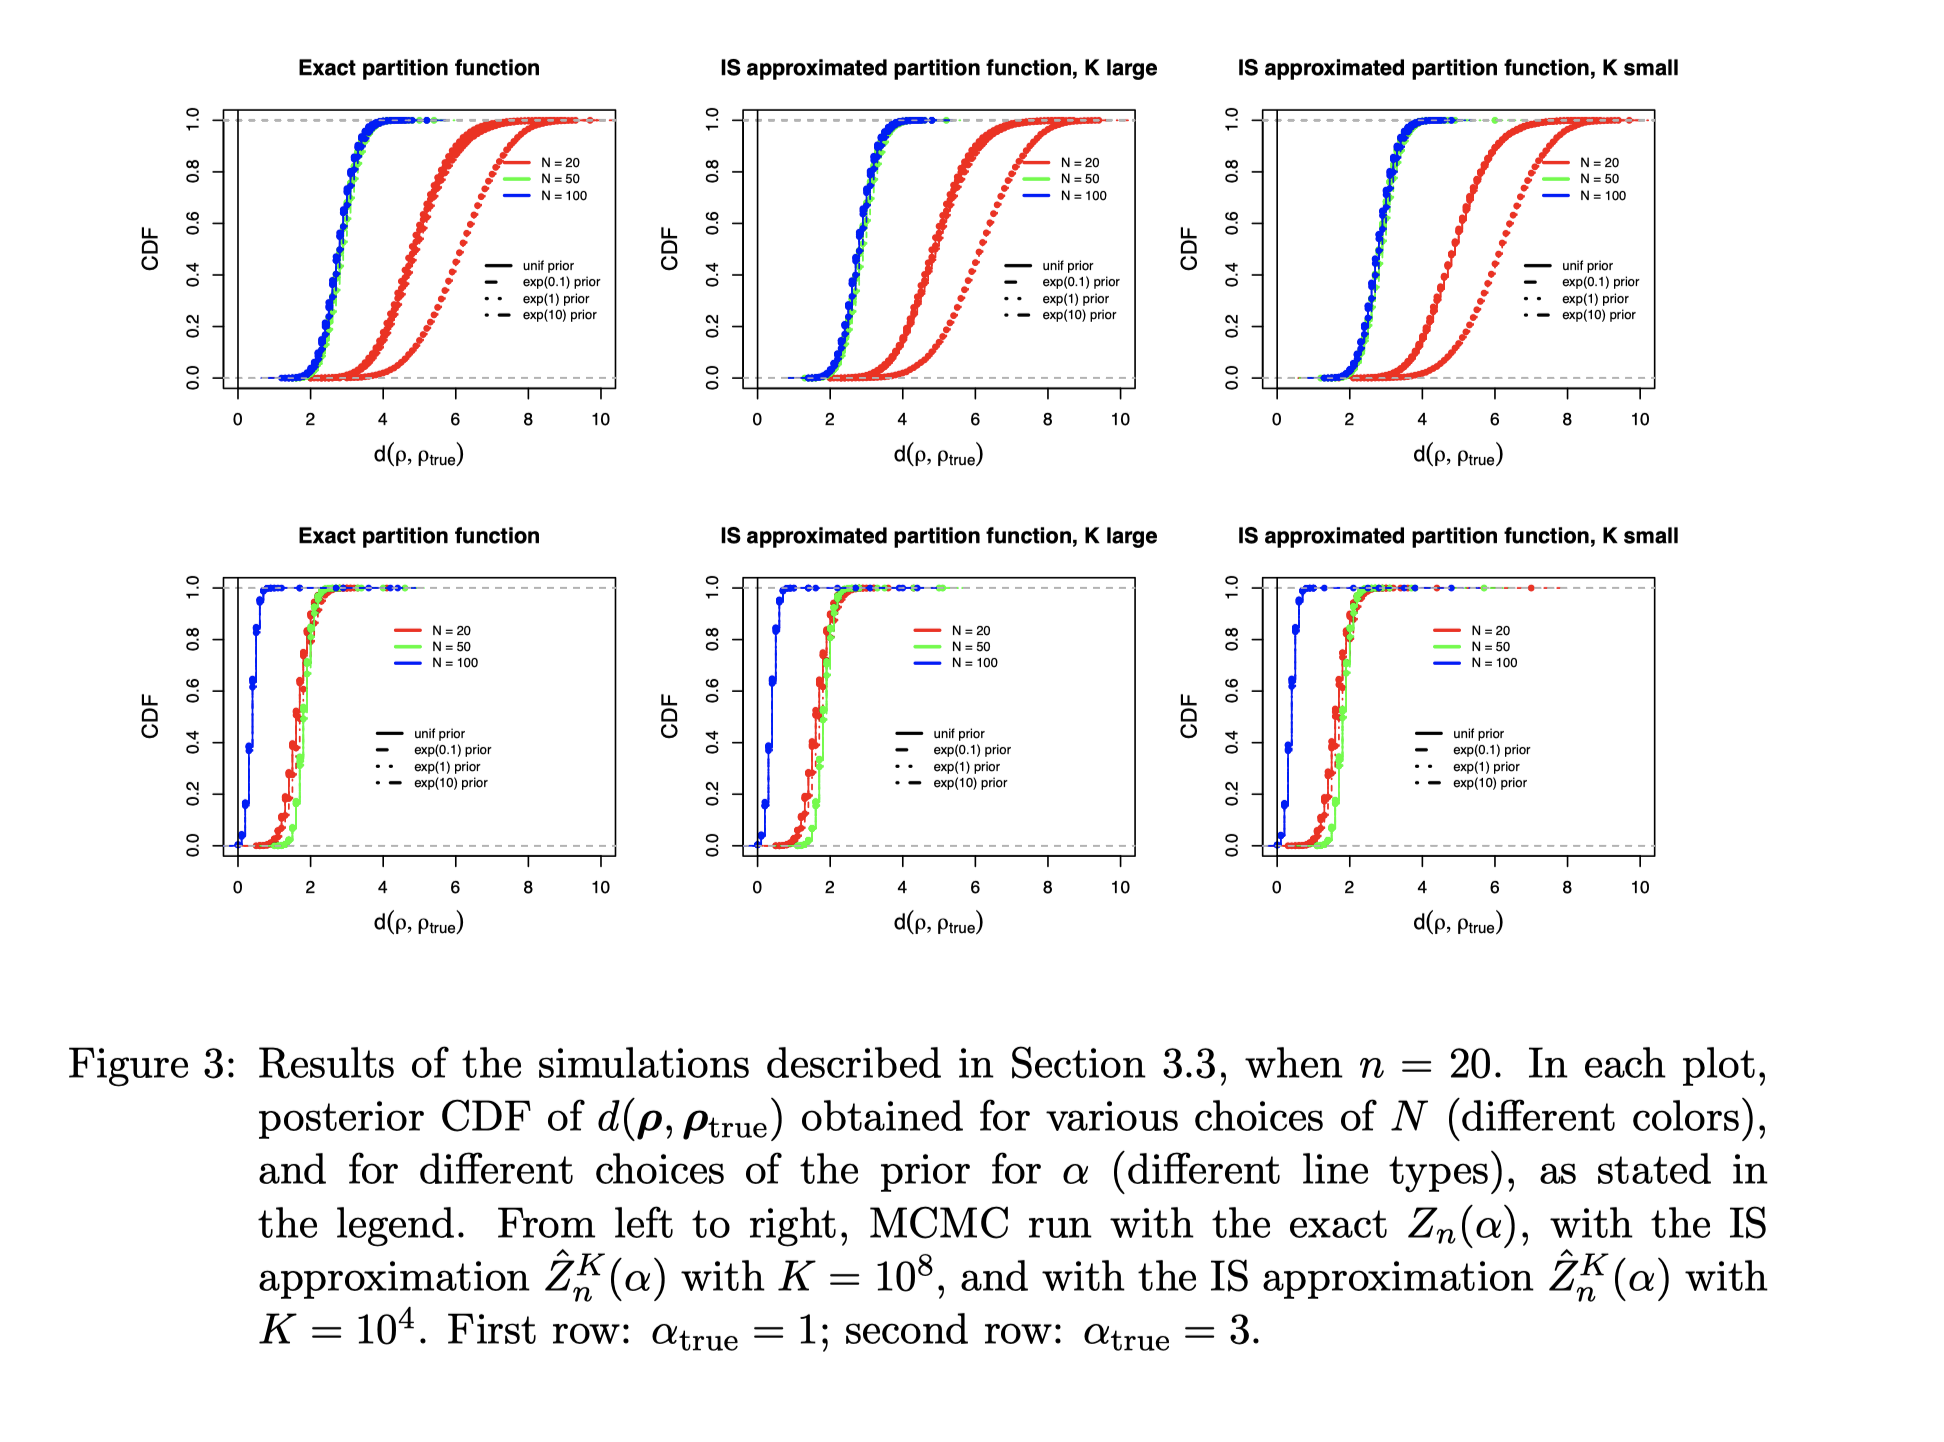
\includegraphics[width=10cm]{VitelliFigure3.png}
    \end{figure}
\end{frame}

\begin{frame}{Studying the effect of approximation by simulations}
\begin{itemize}
    \item Consider the performance of the method when using the IS approximation $\hat Z_n(\alpha)$with $K=10^4$ and $10^8$ then comparing the results with those based on the exact $Z_n(\alpha)$
    \item The precision and the accuracy of the marginal posterior distriutions increasing for $\boldsymbol{\rho}$ with $N$ becoming larger.
    \item For smaller values of $\alpha_{true}$, $\boldsymbol{\rho}$ is stochastically farther from $\rho_{true}$. These results are stable against varying choices of the prior for $\alpha$
    \item Most importantly, inference on $\boldsymbol{\rho}$ is completely unaffected by the approximation of $Z_n(\alpha)$ already when $K=10^4$
    \item Similar results is still yielded when $n$ becomes larger as $50$ or $100$
\end{itemize}
\end{frame}

\begin{frame}{Studying the effect of approximation by simulations}
\begin{itemize}
    \item The main postive result from the perspective of practical applications
    \begin{enumerate}
        \item The relative lack of sensitivity of the posterior inferences to the specification of the prior for the scale parameter $\alpha$
        \item The apprarent robustness of the marginal posterior inferences on $\boldsymbol{\rho}$ on the choice of the approximation of the partition function $Z_n(\alpha)$
    \end{enumerate}
\end{itemize}
\end{frame}

\section{Extensions to Partial Rankings and Heterogeneous Assessor Pool}
\begin{frame}{Assumptions that we will relax in this section}
\begin{itemize}
    \item We will relax two assumptions of the previous sections.
    \begin{enumerate}
        \item Each assessor ranks all $n$ items. 
        \item The assessors are homogeneous, all sharing a common consensus ranking.
    \end{enumerate}
\end{itemize}
\end{frame}

\subsection{Ranking of the Top Ranked Items}
\begin{frame}{Top-$k$ ranks}
\begin{itemize}
    \item Often only a subset of the items is ranked.
    \item These situations can be handled conveninetly in Bayesian framework by applying data augmentation techniques.
    \item We shall consider the case of the top-$k$ ranks.
\end{itemize}
\end{frame}

\begin{frame}{Setting for top-$k$ ranks case}
\begin{itemize}
    \item Among $n$ items $\{A_1, \cdots, A_n\}$, each assessor $j$ has ranked the subset of items $\mathcal{A}_j\subset\{A_1, \cdots, A_n\}$ giving them top ranks from $1$ to $n_j=|\mathcal{A}_j|$. 
    \item Before, we had complete ranking $\mathbf{R}_j\in \mathcal{P}_n$, but now, we denote $\mathbf{R}_j$ as partial ranking.
    \item We have augmented ranking vectors $\tilde{\mathbf{R}}_j\in \mathcal{P}_n$ where unknown part follows a symmetric prior on the permutations of $(n_j+1, \cdots, n)$ for each $j=1, \cdots, N$
\end{itemize}
\end{frame}

\begin{frame}{MCMC Algorithms for top-$k$ ranks case}
\begin{itemize}
    \item $\mathcal{S}_j$ : set of all possible augmented random vectors given original partially ranked items together with the allowable `fill-ins' of the missing ranks, for each $j=1, \cdots, N$
    \item Our goal is to sample from the posterior distribution 
    \begin{equation*}
        P(\alpha, \boldsymbol{\rho}\, |\, \mathbf{R}_1, \cdots, \mathbf{R}_N)=\sum_{\tilde{\mathbf{R}}_1\in \mathcal{S}_1}\cdots \sum_{\tilde{\mathbf{R}}_N\in \mathcal{S}_N}P(\alpha, \boldsymbol{\rho}, \tilde{\mathbf{R}}_1, \cdots,\tilde{\mathbf{R}}_N\, |\, \mathbf{R}_1, \cdots, \mathbf{R}_N )
    \end{equation*}
    \item Our MCMC algorithm alternates between
    \begin{enumerate}
        \item  sampling the augmented ranks given the current values of $\alpha$ and $\boldsymbol{\rho}$
        \item sampling $\alpha$ and $\boldsymbol{\rho}$ given the current values of the augmented ranks.
    \end{enumerate}
    \item The latter is done similar as in Section 2.4, where in this case $\mathbf{R}_1, \cdots, \mathbf{R}_N$ is replaced by $\tilde{\mathbf{R}}_1, \cdots,\tilde{\mathbf{R}}_N$ 
\end{itemize}
\end{frame}

\begin{frame}{MCMC Algorithms for top-$k$ ranks case}
\begin{itemize}
    \item For the former, given the current $\tilde{\mathbf{R}}_j$ (which embeds info contained in $\mathbf{R}_j$) and the current values of $\alpha$ and $\boldsymbol{\rho}$, $\tilde{\mathbf{R}}_j'$ is sampled in $\mathcal{S}_j$ from a uniform proposal distribution which is obviously symmetric.\\ The proposed $\tilde{\mathbf{R}}_j'$ is accepted with probability $\min\{1,r\}$ with 
    \begin{align*}
        r&= \frac{P(\tilde{\mathbf{R}}_1, \cdots, \tilde{\mathbf{R}}_j',\cdots, \tilde{\mathbf{R}}_N\,|\, \alpha, \boldsymbol{\rho})}{P(\tilde{\mathbf{R}}_1, \cdots, \tilde{\mathbf{R}}_j,\cdots, \tilde{\mathbf{R}}_N\,|\, \alpha, \boldsymbol{\rho})} \\ &=\exp[-\frac{\alpha}{n}\big\{d(\tilde{\mathbf{R}}_j', \boldsymbol{\rho})-d(\tilde{\mathbf{R}}_j, \boldsymbol{\rho}) \big\}] 
    \end{align*}
    \item Note that we can generalize this algorithm to generic partial ranking, where items partially ranked by each assessor are not necessarily the top ranked items. 
\end{itemize}
\end{frame}

\begin{frame}{Effects of Unranked Items on the Top-$k$ Consensus Ranking}
\begin{itemize}
    \item It is possible that the number of items is large and there are items which none of the assessors included in their top-list. 
    \item Can we ignore such `left-over' items and consider only the items explicitly ranked by at least one assessor?
    \item The two main points are that
    \begin{itemize}
        \item Only items explicitly ranked by the assessors appear in top positions of the consesnsus ranking.
        \item When considering the MAP(maximum a posteriori) consensus ranking, excluding the left-over items from the ranking procedure already at the start has no effect on how the remaining ones will appear in such consensus ranking.
    \end{itemize}
\end{itemize}
\end{frame}

\begin{frame}{Effects of Unranked Items on the Top-$k$ Consensus Ranking}
\begin{figure}[h]
    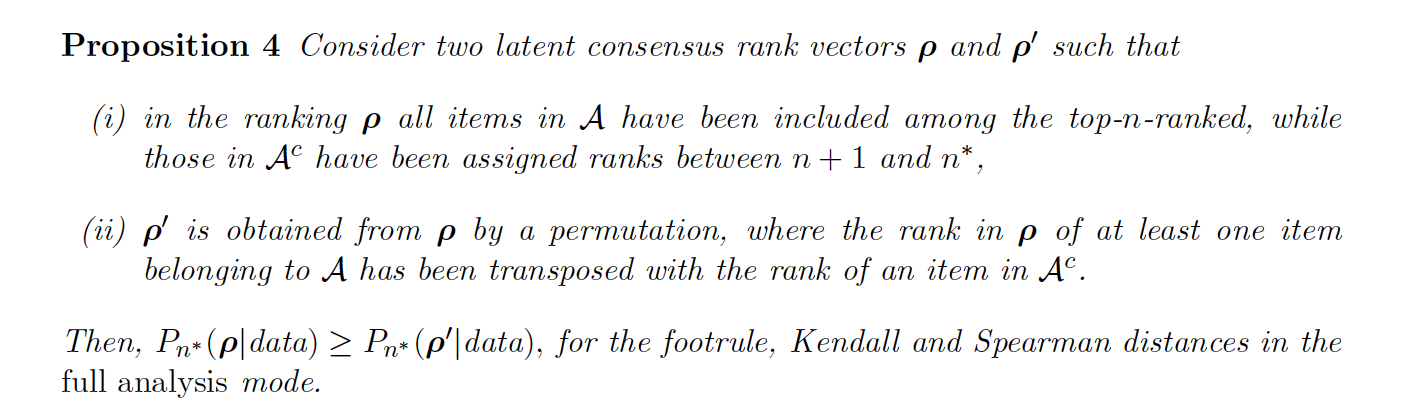
\includegraphics[width=12cm]{Proposition4.png}
    \centering
\end{figure}
\begin{figure}[h]
    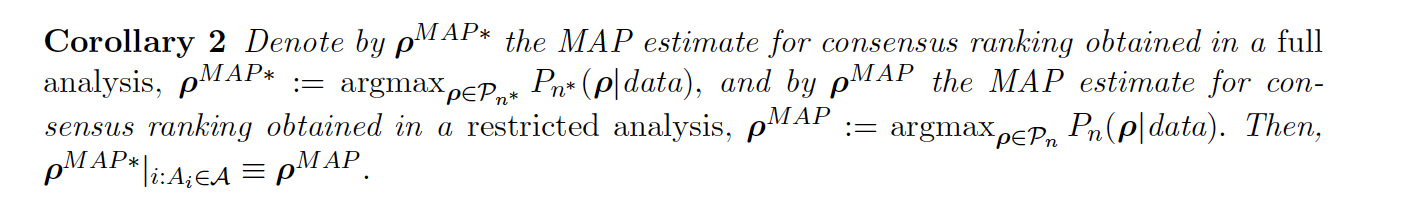
\includegraphics[width=12cm]{Corollary2.png}
    \centering
\end{figure}
\end{frame}

\begin{frame}{Effects of Unranked Items on the Top-$k$ Consensus Ranking}
\begin{itemize}
    \item The above proposition says that the MAP estimate for consensus ranking assigns $n$ highest ranks to explicitly ranked items in the data (Be aware that here we denote the number of total items as $n^*$)
    \item Note that full analysis, which includes the complete set of all  items, cannot always be carried out in practice due to the fact that left-over items might be unknown or too many for realistic computation. The corollary guarantees that the top-$n$ items in the MAP consensus ranking do not depend on whether we include left-over items in the analysis. 
\end{itemize}
\end{frame}

\subsection{Pairwise Comparison}
\begin{frame}{Pairwise Comparison}
\begin{itemize}
    \item Often, assessors compare pairs of items rather than ranking all or a subset of items. 
    \item Notation for pairwise comparison 
    \begin{itemize}
        \item $A_r\prec A_s$ : $A_s$ is preferred to $A_r$, so that $A_s$ has a lower rank than $A_r$ 
        \item $\mathcal{B}_j$ : pairwise orderings or preferences stated by assessor $j$
        \item $\mathcal{A}_j$ : set of items constrained by asessor $j$
        \item $tc(\mathcal{B}_j)$ : the transitive closure of $\mathcal{B}_j$, containing all pairwise orderings of the elements in $\mathcal{A}_j$ induced by $\mathcal{B}_j$.
        \begin{align*}
            \mathcal{B}_j&=\{A_1\prec A_2, A_2\prec A_5\} \\ &\Rightarrow tc(\mathcal{B}_j)=\{A_1\prec A_2, A_2\prec A_5, A_1\prec A_5\} \\\mathcal{B}_k &=\{A_1\prec A_2, A_2\prec A_5, A_4\prec A_5\} \\ &\Rightarrow tc(\mathcal{B}_k)=\{A_1\prec A_2, A_2\prec A_5, A_1\prec A_5, A_4\prec A_5\}
        \end{align*}
    \end{itemize} 
\end{itemize}
\end{frame}

\begin{frame}{MCMC Algorithms for pairwise comparison}
\begin{itemize}
    \item In the MCMC algorithm, we need to propose augmented ranks which obey the partial ordering constraints given by each assessor, to avoid a large number of rejections, with the difficulty that none of the items is now fixed to a given rank.
    \item We can also handle the case when assessors give ties : in such a situation, each pair of items resulting in a ties is randomized to a preference at each data augmentation step inside the MCMC.
\end{itemize}
\end{frame}

\begin{frame}{MCMC Algorithms for pairwise comparison}
\begin{itemize}
    \item The main idea of MCMC algorithm remains the same as the one for the top-$k$ ranks
    \item The difference is that here, a `modified' leap-and-shift proposal distribution, rather than a uniform proposal distribution, is used to sample augmented ranks.
\end{itemize}
\end{frame}

\begin{frame}{Modified Leap-and-Shift proposal}
\begin{itemize}
    \item Only leap step is modified and the shift step remains unchanged.
    \item Given a full augmented rank vector $\tilde{\mathbf{R}}_j$ compatible with $tc(\mathcal{B}_j)$, we shall propose $\tilde{\mathbf{R}}_j'$
    \begin{enumerate}
        \item Draw a random number $u\sim Unif\{1,2,\cdots, n\}$
        \item If $A_u \notin \mathcal{A}_j$ then complete the leap step by drawing $\tilde{R}_{uj}^*\sim Unif\{1,2,\cdots, n\}$
        \item If $A_u \in \mathcal{A}_j$ then complete the leap step by drawing $\tilde{R}_{uj}^*\sim Unif\{l_j+1, \cdots, r_j-1\}$ where $l_j$ and $r_j$ are defined by
        \begin{itemize}
            \item $l_j=\max\{\tilde{R}_{kj} : A_k\in \mathcal{A}_j, k\neq u, (A_k\succ A_u)\in tc(\mathcal{B}_j) \}$ with convention that $l_j=0$ if the set is empty
            \item $r_j=\min\{\tilde{R}_{kj} : A_k\in \mathcal{A}_j, k\neq u, (A_k\prec A_u)\in tc(\mathcal{B}_j) \}$ with convention that $r_j=n+1$ if the set is empty
            \item Briefly, $l_j$ is given rank of the item whose rank is closest to $A_u$ among all assessed items preferred to $A_u$, and $r_j$ is given rank of the item whose rank is closest to $A_u$ among all assessed items less preferred than $A_u$
        \end{itemize} 
    \end{enumerate}
    \item Note that this modified leap-and-shift is symmetric proposal. Hence we use the same acceptance probability as in the top-$k$ ranks case.
\end{itemize}
\end{frame}

\subsection{Clustering Assessors based on their Complete Rankings}
\begin{frame}{Motivation for clustering}
\begin{itemize}
    \item So far we have assumed that there exists a unique consensus ranking shared by all assessors. 
    \item The possibility of dividing assessors into more homogeneous subsets, each sharing a consesnsus ranking of the items, brings the model closer to reality. 
    \item We introduce a mixture of Mallows models to handle heterogeneity.
\end{itemize}
\end{frame}

\begin{frame}{Mixture of Mallows models}
\begin{itemize}
    \item Assume that the data consist of complete rankings.
    \item $z_j\in \{1,\cdots, C\}$ assigns assessor $j$ to one of $C$ clusters for each $j=1,\cdots, N$ \; i.e. $z_1, \cdots, z_N$ are cluster labels.
    \item The assessments $\mathbf{R}$ within each cluster $c\in\{1,\cdots, C\}$ are described by a Mallows model with parameters $\alpha_c$ and $\boldsymbol{\rho}_c$ which is the cluster consensus. 
    \item Assume conditional independence across the clusters.
    \item Likelihood for the observed rankings $\mathbf{R}_1, \cdots, \mathbf{R}_N$ is given by 
    \begin{multline*}
        P(\mathbf{R}_1, \cdots, \mathbf{R}_N|\{\alpha_c, \boldsymbol{\rho}_c\}_{c=1,\cdots, C}, z_1, \cdots, z_N)\\ = \prod_{j=1}^N \frac{1}{Z_n(\alpha_{z_j})}\exp\{-\frac{\alpha_{z_j}}{n} d(\mathbf{R}_j, \boldsymbol{\rho}_{z_j})\}
    \end{multline*}
\end{itemize}
\end{frame}

\begin{frame}{Mixture of Mallows models}
\begin{itemize}
    \item Assumption for priors
    \begin{enumerate}
        \item $\boldsymbol{\rho}_1, \cdots \boldsymbol{\rho}_C \overset{indep}{\sim} \pi_{\boldsymbol{\rho}}$ where $\pi_{\boldsymbol{\rho}}$ is a uniform prior on $\mathcal{P}_n$ as before.
        \item $\alpha_1, \cdots, \alpha_C \overset{indep}{\sim} \pi_\alpha$ where $\pi_\alpha$ is a truncated exponential prior with shared $\lambda$
        \item $\tau_c$ is the probability that an assessor belongs to the c-th cluster. \\ $\tau_c\geq 0 \quad \forall c=1,\cdots, C$ and $\sum_{c=1}^C \tau_c=1$. \; $(\tau_1, \cdots \tau_C)$ are assigned the standard symmetric Dirichlet prior $\mathcal{D}(\psi, \cdots, \psi)$
        \item $P(z_j=c \,|\, \tau_1, \cdots, \tau_C)=\tau_c \quad \forall c=1,\cdots C$ and $z_1, \cdots z_N$ are conditionally i.i.d.
    \end{enumerate}
    \item $\lambda$ and $\psi$ are tuning parameters. What about $C$?
\end{itemize}
\end{frame}

\begin{frame}{How to determine the number of clusters}
\begin{itemize}
    \item The number of clusters $C$ is often unknown, and the selection of $C$ can be based on different criteria.
    \begin{enumerate}
        \item The within cluster sum of distances $\sum_{c=1}^C \sum_{j : z_j=c} d(\tilde{\mathbf{R}}_j, \boldsymbol{\rho}_c)$
        \item The within-cluster indicator of mis-fit to the data \\$\sum_{c=1}^C \sum_{j : z_j=c} \big|\{B\in tc(\mathcal{B}_j):$B is not consistent with $\boldsymbol{\rho}_c\} \big|$ \\
        (valid for pairwise comparison case)
        \item[\rmk] While the former only depends on MCMC outputs $\tilde{\mathbf{R}}_j$ and $\boldsymbol{\rho}_c$ , the latter partly depends on the observed data $\mathcal{B}_j$
    \end{enumerate}
\end{itemize}
\end{frame}

\begin{frame}{How to determine the number of clusters}
\begin{itemize}
    \item Here we use the posterior distribution of the within-cluster sum of distances of the observed ranks from the corresponding cluster consensus.
    \item Separate analyses were performed for $C=1,2,\cdots, \mathcal{C}$ for some $\mathcal{C}$
    \item We expect to observe an `elbow' in the within-cluster distance posterior distribution as a function of $C$, identifying the optimal number of clusters. 
\end{itemize}
\end{frame}

\begin{frame}{MCMC Algorithm for Mixture Mallows model}
\begin{itemize}
    \item The algorithm alternates between 
    \begin{enumerate}
        \item sampling $\boldsymbol{\rho}_1, \cdots, \boldsymbol{\rho}_C$ and $\alpha_1, \cdots, \alpha_C$ in a Metropolis-Hastings step
        \item sampling $\tau_1, \cdots, \tau_C$ and $z_1, \cdots, z_N$ in a Gibbs sampler step.
    \end{enumerate}
    \item The former is straightforward. Update is proceeded element-wisely and the acceptance probability is slightly changed according to the cluster index $c\in \{1,\cdots C\}$
\end{itemize}
\end{frame}

\begin{frame}{Setting for top-$k$ ranks case}
\begin{itemize}
    \item For the latter
        \begin{enumerate}
            \item Gibbs step for $(\tau_1, \cdots, \tau_C)$ \\ Dirichlet prior is conjugate to the multinomial conditional prior. \\ Since $(\tau_1, \cdots \tau_C)\sim \mathcal{D}(\psi, \cdots, \psi)$ \,\& $(n_1, \cdots, n_C)|(\tau_1, \cdots, \tau_C)\sim Multi(N, (\tau_1, \cdots, \tau_C))$ where $n_c=\sum_{j=1}^N I(z_j=c)$ for each $c=1, \cdots ,C$\; , we sample $(\tau_1, \cdots, \tau_C)$ from $\mathcal{D}(\psi+n_1, \cdots, \psi+n_C)$ in the Gibbs step. 
            \item Gibbs step for $(z_1, \cdots, z_N)$ \\ We sample $z_j$ from $P(z_j=c \,|\, \tau, \boldsymbol{\rho}, \alpha, \mathbf{R}_j)\quad \forall c=1, \cdots C$ for each $j=1,\cdots N$ where $\tau, \boldsymbol{\rho}, \alpha$ are $C$-dim vectors. 
            \begin{align*}
                P(z_j=c \,|\, \tau, \boldsymbol{\rho}, \alpha, \mathbf{R}_j) &\propto 
                P(z_j=c\, |\, \tau)P(\mathbf{R}_j \, |\, \boldsymbol{\rho}, \alpha, z_j=c) \\ &\quad \because \text{prior}*\text{likelihood} \\ &= P(z_j=c\, |\, \tau)P(\mathbf{R}_j \, |\, \boldsymbol{\rho}_c, \alpha_c) \\ &= \tau_c Z_n(\alpha_c)^{-1}\exp\Big\{-\frac{\alpha_c}{n}d(\mathbf{R}_j, \boldsymbol{\rho}_c)\Big\}
            \end{align*}
        \end{enumerate}
\end{itemize}
\end{frame}

\begin{frame}{Remark for the extension models}
\begin{itemize}
    \item Merging two algorithms in this section, we can treat situations where incomplete ranking data are observed and assessors must be divided into separate clusters.
\end{itemize}
\end{frame}

\section{Discussion and Examples}
\begin{frame}{Benefit of Bayesian Approach}
\begin{itemize}
    \item Estimation for consensus ranking by MAP estimator
    \item In applications, the interest often lies in computing posterior probabilities of more complex functions of the consensus $\boldsymbol{\rho}$.
    \begin{itemize}
        \item[(Ex)] The posterior probability that a certain item has consensus rank higher than a given level (“among the top 5”, say)
        \item[(Ex)] The posterior probability that the consensus rank of a certain item is higher than the consensus rank of another one. 
    \end{itemize}
    \item Bayesian approach naturally allows to estimate any posterior summary of interest by means of MCMC.
\end{itemize}
\end{frame}

\begin{frame}{Benefit of Bayesian Approach - Preference Prediction}
\begin{itemize}
    \item One such thing is a preference prediction
    \item Situation : assessors have been asked to respond to some queries containing different sets of pairwise comparisons. One may then ask how the assesssors would have ranked for pairwise comparisons when such comparison could not be concluded directly from the data they provided. 
    
\end{itemize}
\end{frame}

\begin{frame}{Benefit of Bayesian Approach - Preference Prediction}
\begin{itemize}
    \item For example, suppose assessor $j$ did not compare $A_1$ to $A_2$. We might be interested in computing $P(A_1\prec_j A_2 \,|\, data)$, the predictive probability that this assessor would have preferred item $A_2$ to item $A_1$. This probability is then readily obtained from the MCMC output as a marginal of the posterior $P(\tilde{\mathbf{R}_j}\,|\,data)$ \\ i.e. If we have $10^5$ MCMC posterior outputs for $\tilde{\mathbf{R}_j}$ then compute the ratio of the number of outputs satisfying $A_1\prec_j A_2$ to the number of total outputs, $10^5$. 
    \item This type of problems is called as preference learning or personalized ranking, which is a step towards personalized recommendation.
\end{itemize}
\end{frame}

\begin{frame}{Example : Sushi Data}
\begin{itemize}
    \item $N=5000$ people were interviewed, each giving a complete ranking of $n=10$ sushi variants.
    \begin{figure}
        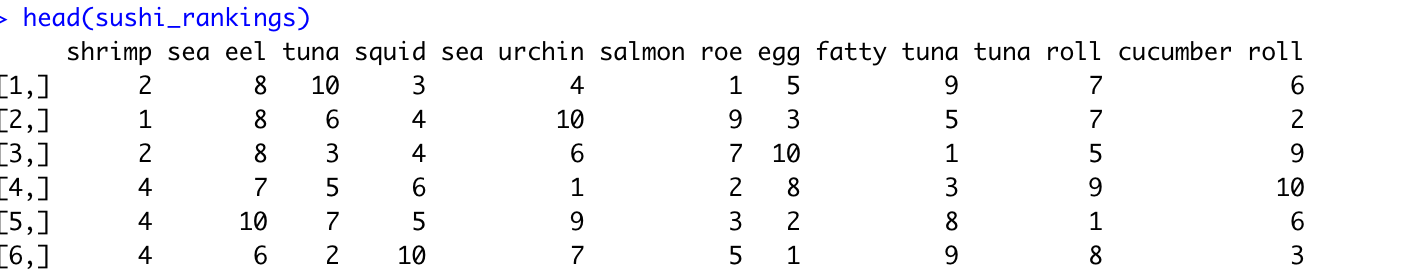
\includegraphics[width=10cm]{sushidata.png}
    \end{figure}
    \item We want to figure out the consensus ranking of sushi.
    \item For convenience, use only a subset of $250$ people.
\end{itemize}
\end{frame}

\begin{frame}{Example : Sushi Data}
\begin{itemize}
    \item Consensus ranking for sushi is estimated as \\
    1. fatty tuna    2. tuna  3. sea eel 4.shrimp 5. salmon roe \\ 6. tuna roll  7. squid   8. sea urchin 9. egg  10. cucumber roll   
    \begin{figure}
        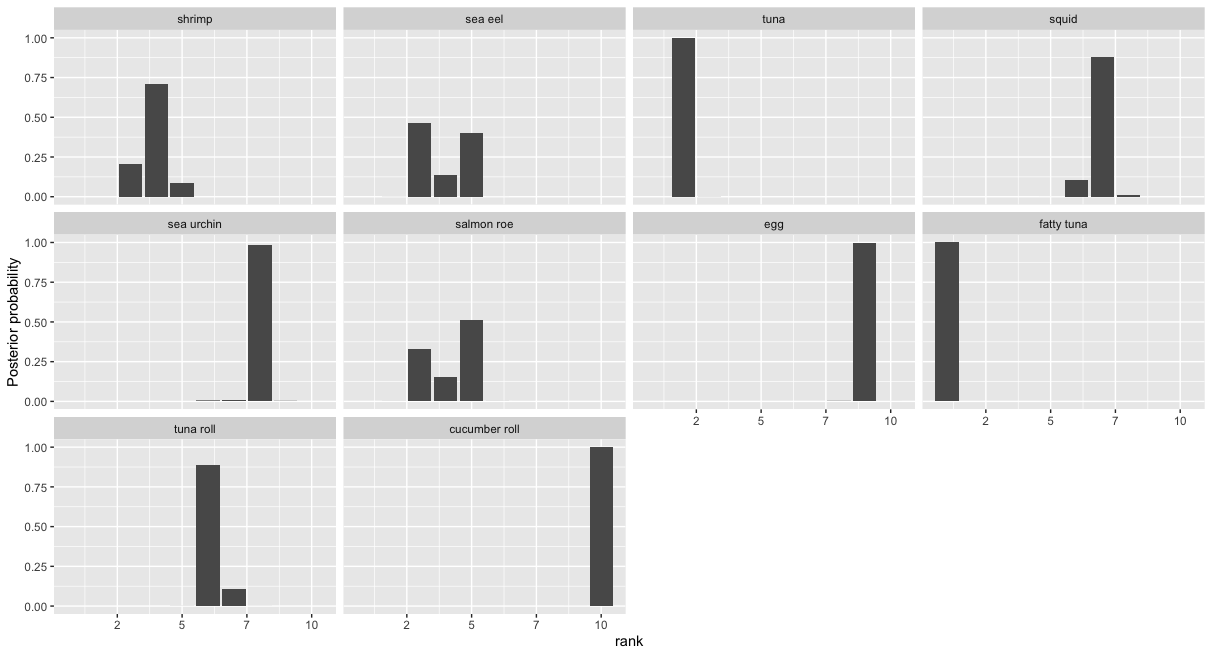
\includegraphics[width=10cm]{Rplot_sushi.png}
    \end{figure}
\end{itemize}
\end{frame}

\begin{frame}{Example : Beach Preference Data}
\begin{itemize}
    \item This is the case in the pairwise comparison
    \item There are $n=15$ images of tropical beaches s.t. they differ in terms of presence of building and people. 
    \item Each assessor answers for comparing a random set of 25 pairs of images. $N=60$ answers are collected. 
    \item Nine assessors returned orderings which contained at least one non-transitive pattern of comparisons. (This refers to the case like $A_1\prec A_2, \, A_2\prec A_3$ but $A_3\prec A_1$).
    \item In this analysis we dropped the non-transitive patterns from the data. Systematic methods for dealing with non-transitive rank data will be considered in another article.
\end{itemize}
\end{frame}

\begin{frame}{Example : Beach Preference Data}
\begin{itemize}
    \item We want to get consensus ranking for beaches and also prediction for the top-3 beaches for each individual.
    \begin{figure}
        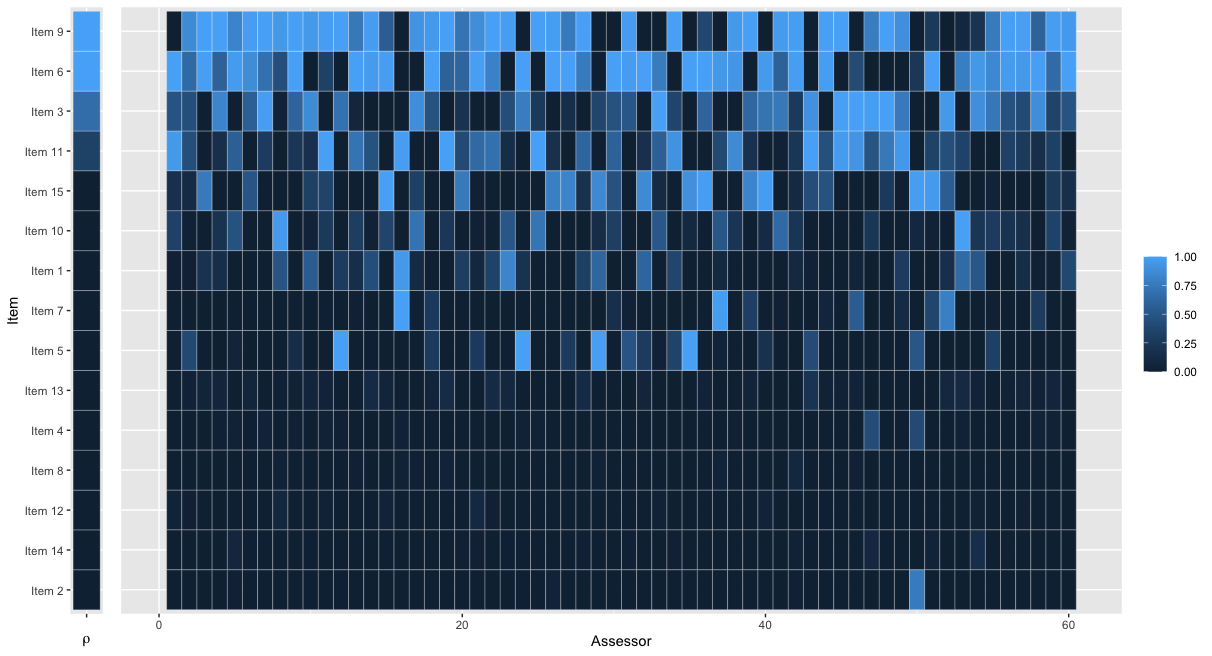
\includegraphics[width=11cm]{Rplot_beach.png}
    \end{figure}
\end{itemize}
\end{frame}

\begin{frame}{Discussion}
\begin{itemize}
    \item The Mallows model performs very well with a large number of assessors $N$
    \item But it may not be computationally feasible when the number of items is extremely large, for example $n\geq 10^4$, which is not uncommon in certain applications. MCMC algorithm converges slowly in such large spaces.
    \item There are many situations where rankings vary over time. We assume to observe ranks at discrete time-points indexed by $t=0,1,\cdots, T$ and let $\boldsymbol{\rho}^{(t)}$ and $\alpha^{(t)}$ denote the parameters of the Mallows model at time t.
    \item A natural generalization of our model is to allow for item-specific $\alpha$'s. The Mallows model with footrule and Spearman distance has not yet been generalized to handle item specific $\alpha$'s mostly due to the obvious computational difficulties. Within our famework, this appears as feasible.  
\end{itemize}
\end{frame}


%\subsection<presentation>*{For Further Reading}
\begin{frame}{Reference}
    \nocite{vitelli2017probabilistic}
    \bibliography{vitelli2017probabilistic}
\end{frame}

\end{document}
